\documentclass[a4paper]{article}

\usepackage[brazil]{babel} % Sumário em PT-BR
\usepackage[utf8x]{inputenc} % reconhecer acentos
\usepackage{listings}
\usepackage{xcolor}
\usepackage{graphicx}

% Para código C++
\lstset{
  belowcaptionskip=1\baselineskip,
  breaklines=true,
  xleftmargin=\parindent,
  language=C++,
  showstringspaces=false,
  basicstyle=\ttfamily\small,
  keywordstyle=\bfseries\color{green!40!black},
  commentstyle=\itshape\color{purple!40!black},
  identifierstyle=\color{blue},
  stringstyle=\color{orange},
  tabsize=2,
}


\begin{document}
\title{Trabalho Integrado}
\begin{titlepage}

\newcommand{\HRule}{\rule{\linewidth}{0.5mm}} % Defines a new command for the horizontal lines, change thickness here

\center % Center everything on the page
 
%----------------------------------------------------------------------------------------
% HEADING SECTIONS
%----------------------------------------------------------------------------------------

\textsc{\LARGE Universidade Federal de São Carlos}\\[1.5cm] % Name of your university/college
\textsc{\Large Trabalho Integrado}\\[0.5cm] % Major heading such as course name
\textsc{\large Programação Orientada a Objetos e Estrutura de Dados I}\\[0.5cm] % Minor heading such as course title

%----------------------------------------------------------------------------------------
% TITLE SECTION
%----------------------------------------------------------------------------------------

\HRule \\[0.4cm]
{ \huge \bfseries Gestão de uma rede de cinemas}\\[0.4cm] % Title of your document
\HRule \\[1.5cm]
 
%----------------------------------------------------------------------------------------
% AUTHOR SECTION
%----------------------------------------------------------------------------------------

\begin{minipage}{0.4\textwidth}
\begin{flushleft} \large
\emph{Autores:}\\
Alessandro V. Piccoli\\
Douglas H. dos Santos\\
Jonathan A. N. da Silva\\
Lucas L. Silva\\
Lucas S. Rocha

\end{flushleft}
\end{minipage}
~
\begin{minipage}{0.4\textwidth}
\begin{flushright} \large
\emph{Registros Acadêmicos:} \\
380105\\
552640\\
489557\\
552321\\
552330

\end{flushright}
\end{minipage}\\[2cm]


{\large Profa. Dra. Katti Faceli}\\
{\large Profa. Dra. Tiemi Christine Sakata}\\[1cm]

%----------------------------------------------------------------------------------------
% LOGO SECTION
%----------------------------------------------------------------------------------------


\includegraphics{logo.png}\\[0cm] % Include a department/university logo - this will require the graphicx package
 
%----------------------------------------------------------------------------------------

\vspace{1cm}
\large {Sorocaba, 30 de Junho de 2014}


\vfill % Fill the rest of the page with whitespace

\end{titlepage}


\tableofcontents

% \pagebreak
\vfill
% \newpage
\addcontentsline{toc}{section}{Lista de Abreviaturas}
\section*{Lista de Abreviaturas}

ABB - Árvore Binária de Busca.\\
AVL - Adelson-Velskii and Landis, árvore binária balanceada.\\
C++ - Linguagem de programação de alto nível desenvolvida por Bjarne Stroustrup nos laboratórios Bell. O C++ acrescenta características orientadas a objeto à linguagem C.\\
CRUD - \textit{Create}, \textit{Read}, \textit{Update} e \textit{Delete}. Traduzindo tem-se: Criar, Ler, Manter e Deletar.\\

\pagebreak


\section{Introdução}
\hspace{5 mm}O programa foi desenvolvido com a finalidade de dar suporte à gestão de um cinema para a empresa \textbf{Faceli \& Sakata Ltda}, esta gerencia uma rede de salas de cinemas. O cenário foi definido de forma que o sistema será desenvolvido por uma segunda empresa: \textbf{Zaina Software}, que é consolidada na área de desenvolvimento de \textit{software}, e já fez produtos para outras redes de cinema no estado de São Paulo.


O programa apresenta como principais funcionalidades: o gerenciamento das salas do cinema, filmes, sessões e vendas de ingressos. Uma rede de cinema pode ter muitas salas de exibição, sendo necessário registrar e manter as informações de cada uma delas (capacidade, número de fileiras e de assentos por fileira junto com a numeração):

\begin{itemize}
\item{Cada sala pode ter um número de fileiras e de assentos por fileira diferentes e pode apresentar um ou mais filmes em diferentes sessões.}

\item{Uma sessão é caracterizada por um filme, uma sala e um horário e tem um número máximo de ingressos que podem ser vendidos de acordo com a capacidade da sala.}

\item{Um ingresso deve conter informações sobre seu tipo: meia entrada ou inteira.}

\item{Um cliente só pode comprar ingressos de sessões ainda não encerradas.}

\item{Uma venda pode ser referente a mais de um ingresso e o comprador pode solicitar vários assentos um ao lado do outro.}

\item{O comprador indica quantos assentos ele quer, e o sistema deve mostrar todas as opções com esse número de assentos consecutivos.}

\item{Quando há algum problema em uma das salas este deve ser registrado.}

\item{Além do gerenciamento, o \textit{software} deve possibilitar a visualização de relatórios.}

\end{itemize}


\pagebreak

\section{Descrição e Diagrama de Classes}
\hspace{5 mm} Considerando o cenário e os requisitos funcionais aprensentados, foi elaborado o diagrama de classes abaixo:\\

\begin{figure}[ht!]
\centering
\advance\leftskip-1.7cm
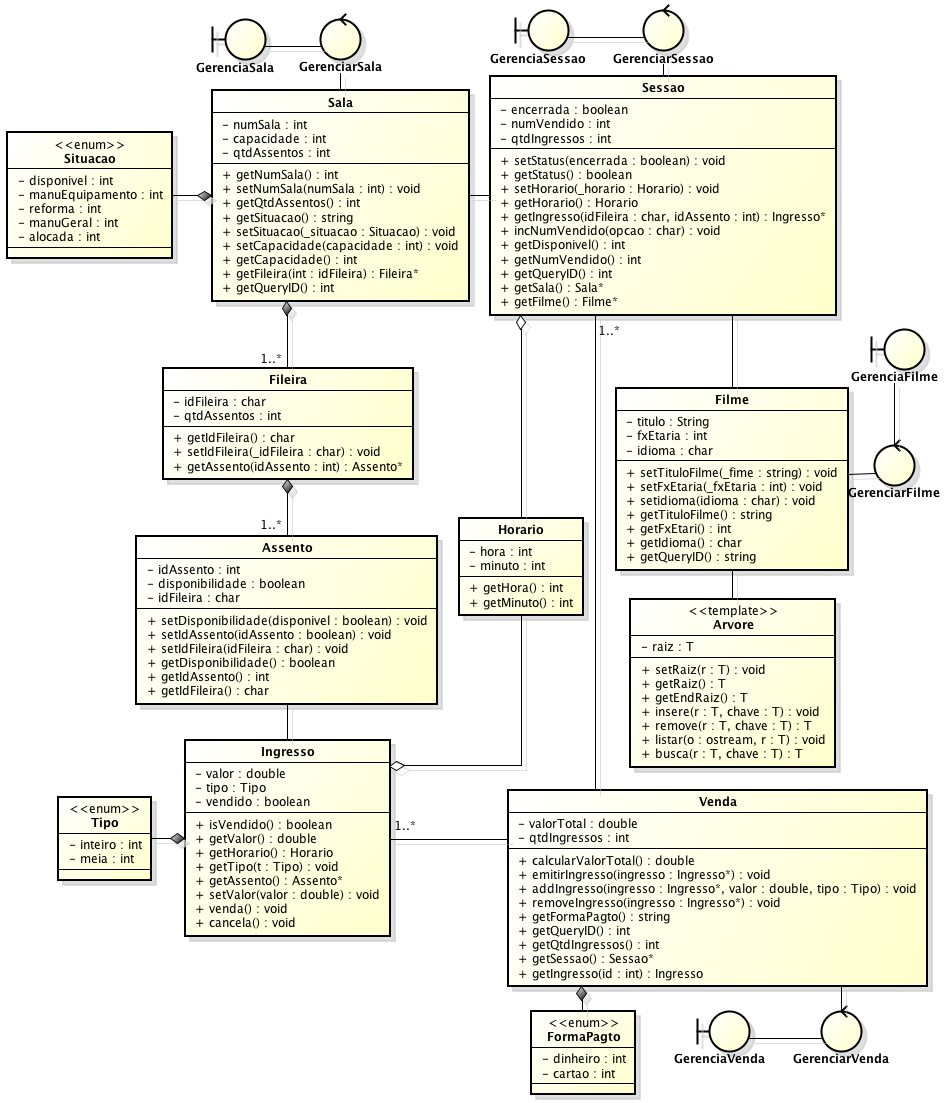
\includegraphics[width=150mm]{diagrama.png}
\end{figure}

%ADD IMAGENS
%\begin{figure}[ht!]
%\centering
%\includegraphics[width=30mm]{fig.png}
%\caption{Recompile}
%\label{fig}
%\end{figure}
%Aqui você pode ver a figura \ref{fig}.

A nossa Equipe foi contratada para fazer a implementação do sistema projetado. Para isso, as seguintes regras foram seguidas:

\begin{itemize}
\item{Todo o tratamento de erros deve ser feito pelo mecanismo de tratamento de exceção;}

\item{O código deve estar bem documentado, e deve ser feita também uma documentação externa;}

\item{Acrescentar os atributos e métodos que forem necessários;}

\item{Ao iniciar e finalizar a execução, o sistema deve recuperar e armazenar em arquivo todos os dados já cadastrados. Empregar os operadores \textless\textless e \textgreater\textgreater;}

\item{Para controlar os objetos das classes, é necessário definir e implementar as estruturas de dados de nossa escolha.}

\end{itemize} 

\section{Como Utilizar o Programa}
\subsection{Menu e Métodos de Entrada}
\hspace{5 mm}O nosso programa foi organizado por menus, onde você escolhe a opção de operação desejada, e o índice encontrado à esquerda da operação representa o número que deverá ser inserido no programa. Qualquer outro número que esteja fora dos especificados no menu não serão aceitos como válidos, e a tela com a lista de operações será reexibida.\\
\quad{\null}\hspace{5 mm}Ao iniciar o programa você encontrará o menu principal, onde poderá estar escolhendo um tipo de gerência dentre as existentes no projeto, através desse menu você poderá realizar desde cadastros de assentos até buscas de filmes, para isso, deverá escolher a sessão correspondente ao tipo de operação que você deseja.\\
\quad{\null}\hspace{5 mm}Após escolher uma das sessões correspondentes, você entrará em um novo menu, onde poderá estar realizando todos os tipos de operações referentes ao CRUD da sessão, podendo ser este desde cadastro de uma nova venda, busca de salas, listagem de sessões ou remoção de filmes. As quatro operações estarão disponíveis a todos so tipos de gerenciamento.\\

\subsection{Tipos de Operações:}
\begin{itemize}
\item{Criar: você poderá estar criando um novo objeto ou serviço através dessa operação. É importante ter conhecimento de que, para muitos serviços, é necessário haver ao menos 1 cadastro de algum objeto, um exemplo é no caso de pesquisar uma sessão que não existe, ou efetuar uma venda sem filmes cadastrados. Dependendo do tipo de cadastro a entrada pode ser diferente, variando entre caracteres ou algarismos, por isso é importante estar atento ao que é requisitado na hora do cadastro, e ser inserido os dados corretos, para que não haja problemas de busca ou remoção futuramente.}
\item{Remover: como o nome já diz, esta operação remove algum dado ou objeto cadastrado no sistema. Uma observação importante é que, assim como você não possui nenhum cadastro no início do programa, não podendo assim efetuar operações como busca. Caso você remova por completo algum objeto (remover todos os filmes por exemplo), você também entrará na situação descrita, onde determinados serviços estarão indisponíveis.}
\item{Buscar: você poderá sempre imprimir na tela a lista de operações ou servidos cadastrados ou calculdaos. Mesmo os dados sendo salvos nos arquivos ".data", é de crucial importância que seteja disponível a exibição das informações durante a execução do programa, para isso essa operação foi desenvolvida e estará sempre ativa (mas nem sempre disponível, como descrito anteriormente é necessário que algumas condições sejam efetivadas para o funcionamento correto).}
\item{Editar: após algum tipo de cadastro, pode ser que informações tenham sido inseridas incorretamente e seja necessário corrigi-las, para que não o usuário não precise remover e cadastrar novamente os dados, criamos um menu para edição de informações no sistema. Após a edição ser finalizda, os dados são atualizados tanto no software (enquanto este está sendo executado) como nos arquivos ".data", onde os novos valores serão salvos.}
\item{Listar: um fato importante em qualquer projeto, é como e quando poderão ser exibidos relatórios para o usuário. No nosso projeto é possível exibir uma lista de todos os objetos e serviços cadastrados, uma forma de relatório, onde é o usuário acompanha o avanço do funcionamento e cadastros no programa. Cada gerenciador terá a sua listagem separada, exibindo os dados pertinentes ao mesmo. Como em outros casos ja descritos, apenas serão exibidos relatórios de informações ja cadastradas, caso não exista nenhum serviço ou objeto cadastrado, o comando de listagem não será executado e um alerta será exibido.}
\end{itemize}

\pagebreak

\section{Implementações}
\hspace{5 mm}O projeto foi desenvolvido em linguagem C++, utilizando o paradigma orientado a objetos, possibilitando assim a modelagem do projeto em classes as quais permitem uma visão do sistema semelhante à uma visão do mundo real de um cinema. Utilizaremos estas classes para realizar os procedimentos necessários na venda de ingresssos e gerenciamento do cinema em geral.\\
\quad{\null}\hspace{5 mm}A seguir listaremos as classes utilizadas no projeto, uma descrição simples sobre cada uma delas (papel no sistema e comportamento) e por fim o algoritmo da classe criada pelo Grupo (\textit{header}).

\subsection{Classe Sessão}
\hspace{5 mm}A Sessão é uma das classes mais importantes do projeto, responsável, de certo modo, pelo gerenciamento geral do projeto. Está conectada à todos os "braços" do diagrama de classes, se relacionando, direta ou indiretamente, com a maioria das classes envolvidas no projeto.\\
\quad{\null}\hspace{5 mm}Podemos dizer que é a estrutura base para o projeto, possuindo maior parte da informação necessária (através dos ponteiros que permitem que esta classe conheça muitas outras) para realização das vendas e controle dos dados.\\
\quad{\null}\hspace{5 mm}Como é possível ver, utilizamos métodos para manipulação das informações e relacionamentos entre as classes que estão de alguma forma relacionadas à esta classe.

\subsubsection{Algoritmo Desenvolvido}
\lstinputlisting{headers/sessao.h}

\pagebreak

\subsection{Classe Sala}
\hspace{5 mm}A classe Sala gerencia as informações referentes a cada sala dentro do cinema. É composta pela classe Fileira (relação 1 para muitos), criando também um vetor de ponteiros para Fileira ao ser criada. Possui os dados referentes à situação e capacidade das salas. Uma sala também tém conhecimento da disponibilidade de cada assento que pertence a cada fileira que a compõe.\\

\subsubsection{Algoritmo Desenvolvido}
\lstinputlisting{headers/sala.h}

\pagebreak

\subsection{Classe Fileira}
\hspace{5 mm}A classe Fileira é a responsável pela criação dos assentos que formam uma sala.\\
\quad{\null}\hspace{5 mm}Com essa classe podemos recolher todas as informações sobre cada assento através do método getAssento(), para depois enviar estas informações para a classe Sala.

\subsubsection{Algoritmo Desenvolvido}
\lstinputlisting{headers/fileira.h}

\pagebreak

\subsection{Classe Assento}
\hspace{5 mm}Classe capaz de instanciar todos os assentos de cada fileira da sala. Quando um ingresso é vendido, é esta classe que altera a situação do assento referente à este ingresso através dos métodos de gerenciamento da disponibilidade. A partir da disponibilidade de cada assento podemos analisar a disponibilidade da fileira, e a partir desta ver o ocupamento da sala.\\

\subsubsection{Algoritmo Desenvolvido}
\lstinputlisting{headers/assento.h}

\pagebreak

\subsection{Classe Filme}
\hspace{5 mm}A classe Filme é responsável pelo gerenciamento de cada filme cadastrado. Estes objetos possuem todas as informações necessárias para a descrição de um filme, tais como título, faixa etária, idioma, etc.\\
\quad{\null}\hspace{5 mm}Para instanciar o conjunto de filmes existentes em nosso cinema, foi utilizado um \textit{template} da estrutura de dados ABB desenvolvido pelo nosso Grupo. A justificativa para o uso desta estrutura de dados é o fato dela permitir buscas em tempo otimizado, além de ser capaz de manter os filmes em ordem alfabética por natureza, sem necessidade de utilizar algoritmos de ordenação, o que é muito interessante em termos de complexidade.

\subsubsection{Algoritmo Desenvolvido}
\lstinputlisting{headers/filme.h}

\pagebreak

\subsection{Classe Ingresso}
\hspace{5 mm}Esta é outra classe com grande importância dentro do projeto, por estar ligada à diversas outras classes. Cada objeto desta classe possui toda informação necessária sobre os ingressos que são vendidos e emitidos no cinema.\\
\quad{\null}\hspace{5 mm}Como pode ser visto no Diagrama de Classes, esta classe se relaciona diretamente com a Venda (pois cada venda realizada é de um ou mais ingressos, que possuem as informações de um assento para o cliente, com isso, podemos ver claramente a ligação com a classe Assento), mas além desta, é necessário um relacionamento com a classe Sessão, pois, segundo nosso \textit{design} de projeto, quando uma sessão é instanciada, automaticamente geramos os ingressos relativos à todos assentos da sala que esta sessão aloca, e a disponibilidade destes é atualizada sempre que realizamos uma venda\\
\quad{\null}\hspace{5 mm}Os métodos venda() e cancela() desta classe se relacionam diretamente com o assento referente a cada ingresso. Ao chamar venda(), mudamos o status deste assento para ocupado, e ao chamar cancela(), fazemos este assento voltar a ser disponível. Estes métodos são disparados sempre que a classe Venda solicita uma adição ou remoção de ingresso.

\subsubsection{Algoritmo Desenvolvido}
\lstinputlisting{headers/ingresso.h}

\pagebreak

\subsection{Classe Venda}
\hspace{5 mm}A responsabilidade principal de um objeto da classe Venda é obter as informações referentes à uma única venda (que pode conter vários ingressos), enviar informações para o controle das sessões (disponibilidade de assentos), e enviar mensagens para todos ingressos relativos à esta venda contendo informações como tipo do ingresso e valor.
\quad{\null}\hspace{5 mm}

\subsubsection{Algoritmo Desenvolvido}
\lstinputlisting{headers/venda.h}

\pagebreak

\subsection{Classe Horario}
\hspace{5 mm}Esta classe foi criada com o intuito de implementar uma definição simples e robusta de um horário. Ela conta com apenas dois atributos, hora e minuto, que definem um horário, e também conta com sobrecargas feitas especialmente para ler e imprimir horários no formato HH:MM, que é muito intuitivo para qualquer usuário do sistema.

\subsubsection{Algoritmo Desenvolvido}
\lstinputlisting{headers/horario.h}

\pagebreak

\subsection{Boundary GerenciaSessao}
\hspace{5 mm}Boundary responsável por gerenciar a classe Sessao, seja para criar ou remover uma sessão ou salvar as informações cadastradas no arquivo ".data", no qual estaremos realizando o \textit{backup} das informações fornecidas de forma organizada, nos perditindo trablahar de maneira mais segura e eficiente.\\
\quad{\null}\hspace{5 mm}Como pode ser observado pelo algoritmo a seguir, os métodos compostos nessa boundary são de grande maioria referentes ao CRUD da classe Sessao, assim como os atributos são ponteiros usados para gerenciar a memória que será usada para salvar as informações da classe (referentes à sala e filme).
\subsubsection{Algoritmo Desenvolvido}
\lstinputlisting{headers/gerenciasessao.h}

\pagebreak

\subsection{Boundary GerenciaSala}
\hspace{5 mm}Boundary responsável por gerenciar a classe Sala, tendo o mesmo propósito que o boundary descrito anterimente, este é usado para o CRUD da sala, criando, removendo, buscando ou editando informações da classe.\\
\quad{\null}\hspace{5 mm}Os atributos usados nesse boundary por sua vez, não se restringem apenas à ponteiros, onde iremos armazenar as informações de cada sala, mas também uma variável com a quantidade de salas, utilizada para maior administração da classe.
\subsubsection{Algoritmo Desenvolvido}
\lstinputlisting{headers/gerenciasala.h}

\pagebreak

\subsection{Boundary GerenciaVenda}
\hspace{5 mm}A classe de vendas, sendo uma das que recebe maior movimento de informações, também possui um boundary, necessário para que cada venda aconteça sem problemas.\\
\quad{\null}\hspace{5 mm}Quando se realiza uma venda é necessário estarmos atentos a vários fatores importantes, que variam dos assentos ao ingresso em si, por isso a classe é composta por métodos para adicionar ingressos à venda, e nos atributos possuimos o espaço preparado na meḿoria para o armazenamento das informações, uma variável para controle da quantidade de vendas realizadas e um ponteiro para o boundary da Sessão, pois este possui informações sobre todo o cinema, muitas vezes essencial para que a venda ocorra.
\subsubsection{Algoritmo Desenvolvido}
\lstinputlisting{headers/gerenciavenda.h}

\pagebreak

\subsection{Boundary GerenciaFilme}
\hspace{5 mm}O grupo concordou que seria de grande utilizade o desenvolvimento de um boundary para a classe Filme, pelo simples fato de que cada filme possui um CRUD, e este deve ser organizado e administrado de forma clara e prática, possibilitando o cadastro ou exclusão de filmes com métodos específicos, além é claro, de atributos que proporcionem o armazenamento e a organização das informações na memória de forma segura.\\
\quad{\null}\hspace{5 mm}É importante ressaltar que os dados estão sendo armazenados em arquivos ".data", onde as informações podem ser consultadas e salvas de maneira prática.
\subsubsection{Algoritmo Desenvolvido}
\lstinputlisting{headers/gerenciafilme.h}

\pagebreak

\section{Estrutura de Dados Usada}
\hspace{5 mm}Durante o projeto, utilizamos alguns métodos aprendidos em sala para gerenciamento dos dados, principalmente quanto à parte de busca, onde utilizamos árvores binárias de busca para manter os filmes do cinema e permitir que as operações sobre estes filmes sejam eficientes (buscas em ABB possuem eficiência da ordem de O(\textit{log n}), e quanto ao armazenamento, onde discutimos os métodos mais fáceis e eficazes nos casos que trabalhamos, tanto para informações inseridas pelo usuário como dados gerenciados durante a execução do projeto.\\


O arquivo \textbf{Arvore.h} representa um \textit{template} de ABB com métodos de inserção, remoção, busca e listagem \textit{inorder}, lembrando que este último realiza a impressão ordenada devido à própria natureza de uma ABB. No caso dos filmes, a ordem é dada pela ordem lexicográfica dos títulos.\\

Foi considerado o uso da estrutura de árvore AVL devido ao auto-balanceamento deste tipo de árvore, que permite uma eficiência ainda maior nas buscas. Porém, por dificuldade de implementação, e devido ao fato de o ganho de eficiência não ser muito grande, foi mantida a utilização das árvores ABB, cuja implementação é bem mais simples.
\pagebreak

\section{Como Compilar}
\hspace{5 mm}Para facilitar a compilação, utilizamos um Makefile que reconhece todos os arquivos de implementação necessários (.cpp) e os compila automaticamente. Basta usar o comando make no terminal. Ao finalizar a compilação, será gerado um executável nomeado "cinema.exe". Para desinstalá-lo, basta usar o comando make uninstall.\\
O funcionamento do Makefile é explicado a seguir.

\begin{enumerate}
\item{Variáveis}\\
Nós criamos duas variáveis antes de executar as targets no algoritmo. Primeiramente utilizamos a "CC", que estará recebendo como parâmetro uma referência indicando o tipo de compilador que será necessário para a criação do arquivo executável do nosso projeto, sendo neste caso, o compilador "g++", pois estamos compilando um algoritmo desenvolvido em C++. Em segundo lugar utilizamos de uma variável "EXE", que recebe uma string para o nome do arquivo de output da compilação do projeto.

\item{Target referenciando arquivo de output}\\
Nessa fase do Makefile, nós estamos referenciando nossa variável que contém o arquivo de output e a target "clean", para limpeza do diretório.

\item{Execução da Compilação}\\
Após os procedimentos descritos anteriormente, estamos prontos para realizar enfim a compilação. Primeiramente nós chamamos a variável "CC" com o tipo de compilador a ser usado e declaramos a pasta onde estão todos os arquivos ".cpp". Segundo nós realizamos o mesmo tipo de operação com a classe "main", cujo pré-requisito é a necessidade de ja possuir todas as outras classes ja compiladas e prontas para uso. Quando executamos essa parte do Makefile é gerado o arquivo executável, tornando nosso projeto pronto para ser usado.

\item{Target Clean}\\
Dentro dessa target nós especificamos os comandos necessários para limpar um arquivo, removendo todos os arquivos objeto (*.o) das bibliotecas, além de arquivos temporários (~). É importante lembrar que após a execução da compilação essa target é executada automaticamente.

\item{Target Uninstall}\\
Essa target é apenas um acréscimo ao nosso Makefile, tornando possível a desinstalação do arquivo executável. Sua chamada não é implícita, portanto para ser utilizado basta escrever "uninstall" após a chamada do Makefile.

\end{enumerate}

\pagebreak

\subsection{Makefile}
\lstinputlisting{headers/Makefile.h}

\pagebreak

\section{Decisões de Projeto}
\hspace{5 mm}Durante a implementação do projeto, nosso Grupo realizou diversas decisões relacionadas à modificações na estrutura. Estas decisões foram realizadas tanto em partes da estrutura geral do projeto (diagrama de classes) como em classes específicas (interface e responsabilidades de cada classe).\\
\quad{\null}\hspace{5 mm}Com estas decisões pudemos criar um projeto mais detalhado e organizado, com operações mais controladas e eficazes.\\
\quad{\null}\hspace{5 mm}Iremos descrever a seguir cada uma das decisões, seguidas pela especificação de qual parte do projeto elas foram implementadas e o porque de cada decisão tomada.

\subsection{Referentes à Classe Assento}
\begin{enumerate}

\item{Atributo Disponibilidade}\\
Realizamos a troca do tipo do atributo de Inteiro para Booleano, pois haverá apenas dois casos possíveis - disponível ou não disponível.

\item{Complemento dos atributos idAssento, idFileira e Disponibilidade}\\
Acrescentamos os métodos get e set para todos os atributos.

\end{enumerate}

\subsection{Referentes à Classe Fileira}
\begin{enumerate}

\item{Observação quanto ao Construtor}\\
Construtor irá definir quantidade de assentos nas fileiras.

\item{Atributo qtdAssentos}\\
Decidimos fazer a criação de um novo atributo responsável pela quantidade de assentos em uma fileira.

\item{Método getAssento}\\
Utilizamos o método para retornar o endereço de um determinado assento.

\end{enumerate}

\subsection{Referentes à Classe Filme}
\begin{enumerate}

\item{Criação da Classe}\\
Observando o diagrama de classes, decidimos que seria uma boa ideia para o desenvolvimento do projeto que fosse criado uma classe separada "Filmes", onde estariam localizadas todas as informações sobre cada filme cadastrado.

\end{enumerate}

\subsection{Referentes à Classe Horario}
\begin{enumerate}

\item{Criação da Classe}\\
Criamos a classe Horario porque algumas classes - Ingresso e Sessao - têm que ter o horario.

\end{enumerate}

\subsection{Referentes à Classe Ingresso}
\begin{enumerate}

\item{Atributo horaIngresso}\\
Armazena o horário referente ao ingresso.

\item{Métodos venda e cancela}\\
Atualizam a disponibilidade do assento.

\end{enumerate}


\subsection{Referentes à Classe Sala}
\begin{enumerate}

\item{Atributo qtdAssentos}\\
Define quantos assentos as fileiras devem ter. Todas as fileiras terão necessariamente a mesma quantidade de assentos sempre.

\item{Atributo capacidade}\\
Atributo utilizado para definir a quantidade de fileiras na sala, delimitando assim a capacidade total da sala por capacidade*qtdAssentos.

\item{Método getFileira}\\
Utilizamos o método para retornar o endereço de uma determinada fileira.

\end{enumerate}

\subsection{Referentes à Classe Sessão}
\begin{enumerate}  

\item{Atributo encerrada}\\
Realizamos a troca do tipo do atributo de Inteiro para Booleano, pois haverá apenas dois casos possíveis (encerrada ou não encerrada).

\item{Atributo horario}\\
Decidimos por utilizar um único horário por sessão ao invés de arrays, por questão de simplicidade. Portanto, filmes que são exibidos em mais de um horário devem possuir multiplas sessões.

\item{Consideração em relação ao filme}\\
Decidimos criar uma classe Filme ao invés de usar um unico atributo filme. Esta classe armazena tanto o nome do filme quanto a faixa etária e o idioma.

\item{Métodos getSala e getFilme}\\
Estes métodos retornam o endereço da sala e do filme associados a uma determinada sessão.

\end{enumerate}

\subsection{Referentes à Classe Venda}
\begin{enumerate}

\item{Atributo dtVenda}
O atributo foi removido da classe.

\item{Métodos emitirIngresso e removeIngresso}\\
A assinatura dos métodos foi alterada para receber um ponteiro para um ingresso, ao invés de um objeto da classe Ingresso.

\item{Método addIngresso}\\
A assinatura do método foi alterada para receber um ponteiro para um ingresso, alem de seu valor e tipo.

\item{Método getSessao}
Retorna o endereço da sessão relativa a uma determinada venda.

\item{Método getIngresso}
Retorna o endereço de um ingresso, de acordo com o id fornecido como parâmetro.

\end{enumerate}

\subsection{Referentes às Classes com Boundary}
Todas as classes que possuem um Boundary, há um QueryID referente aos atributos usados para buscar um objeto.

\pagebreak

\section{Dificuldades no Projeto}
\hspace{5 mm}Durante o desenvolvimento do projeto, devido ao pouco tempo de implementação efetiva com a linguagem C++, tivemos algumas dificuldades relativas à sintaxe e uma implementação adequada que mantesse o encapsulamento de todas as classes, acessando seus atributos e mantendo suas alterações como esperado.\\

Além disso, houve dificuldade em relação à escolha das estruturas de dados que seriam potencialmente necessárias para nosso projeto. Foi cogitada a utilização de listas ligadas e de árvores AVL, porém, por simplicidade, fizemos uso apenas de árvores ABB. De qualquer forma, vale citar que o uso de árvores AVL para manter a busca de salas, sessões e filmes seria viável e interessante.


\pagebreak

\section{Testes Realizados}
\hspace{5 mm}Para testar todas as funcionalidades do sistema, simulamos uma execução em que adicionamos uma sala, uma sessão, alguns filmes (sendo que um destes é relativo à sessão criada), e uma venda de alguns ingressos para esta sessão. Mais detalhes sobre os testes realizados, e novos testes presenciais serão realizados durante a apresentação do projeto.

\pagebreak

\section{Conclusão}
\hspace{5 mm}Este trabalho integrado nos proporcionou uma experiência de se trabalhar em grupo, dividindo as responsabilidades, assim como num ambiente empresarial, que enfrentaremos no mercado de trabalho futuramente. Para isto utilizamos um repositório privado no servidor do GitHub, onde todos os membros poderiam ter acesso e onde conseguiríamos um controle de versões.\\

Durante esta forma de trabalhar, que é nova para alguns de nossos integrantes de projeto, pudemos perceber o quanto os conceitos de programação orientada a objetos são comuns no dia-a-dia e são de extrema importância para a modelagem de problemas do mundo real em sistemas de informação, reúso de código, separação de responsabilidades e divisão da estrutura de um projeto.\\

Conseguimos aplicar os conhecimentos passados em sala de aula de forma efetiva e em uma situação real, aplicando, assim, todos os conceitos de programação orientada a objetos dentro de um sistema que lida com a realidade, mostrando a sua importância e implementação.\\

Tais fatores auxiliaram no aprendizado dos conceitos básicos aprendidos durante o semestre e permitiram com que adquiríssemos maior entendimento da linguagem e conhecimento de forma geral.\\

Outro ponto muito positivo foi o estímulo de se trabalhar com um grupo unido e com um mesmo foco, e quando o objetivo é cumprido, dividir este sucesso de um projeto funcional é extremamente gratificante.

\pagebreak

\section{Bibliografia}

\begin{thebibliography}{x}

\bibitem{Aguilar} AGUILAR, LUÍS J. – Programação em C ++: algoritmos, estruturas de dados e objetos – Porto Alegre: McGraw Hill, 2008.

\bibitem{Deitel} HARVEY M. – C++ como programar – 5ed. São Paulo: Pearson, 2006.

\bibitem{Faceli} FACELI, K. Slides de aula – Programação Orientada a Objetos, 2014.

\bibitem{Horstmann} HORSTMANN, C. – Conceitos de computação com o essencial de C++ – 3ed. Porto Alegre: Bookman, 2005.

\bibitem{Sutter}SUTTER H. – Programação avançada em C++ – 1ed. São Paulo: Pearson, 2006. 

\end{thebibliography}

\end{document}